\documentclass[12pt, a4paper]{article}
\usepackage{graphicx}
\usepackage{mathtools}
\usepackage{xcolor}
\usepackage{amsmath}
\usepackage{caption}
\usepackage[italian]{babel}
\usepackage{eso-pic}
\usepackage{setspace}
\usepackage{multirow}
\usepackage{array}
\usepackage{geometry}
\usepackage{longtable}
\graphicspath{ {./immagini/} }
\linespread{1.1}
\geometry{
 total={170mm,257mm},
 left=20mm,
 top=15mm,
 bottom=28mm
 }
 
 \title{\textbf{\scalebox{1.3}{\text{Caduta libera}}}}
 \date{}

\begin{document}
\maketitle
\AddToShipoutPictureBG*{%
  \AtPageUpperLeft{%
    \hspace{\paperwidth}%
    \raisebox{-\baselineskip}{%
      \makebox[0pt][r]{\textbf{Gruppo 10}: Mussini Simone, Ruscillo Fabio, Musi Francesco}}}}%


\section{Cose da aggiungere}
\begin{itemize}
    \item Foto scattate da noi dell'apparato sperimentale
    \item grafici di risultati sbagliati
    \item tabelle dei dati utilizzati (messe subito dopo dire che calcoli fare)
    \item scrivere "Gruppo $10$" vicino ai nomi
    \item mettere i nomi e il gruppo in alto a sinistra ( e non sotto al titolo)
    \item spiegazione generale con formule (ma non troppo) di quale fenomeno fisico andiamo ad osservare
    \item SCRIVERE DELLE CONCLUSIONI LUNGHE E DETTAGLIATE (ho visto dalla relazione che ha consegnato Fra che il prof ha detto che dovevno essere più lunghe (erano di mezza pagina se non di più))
    \item I grafici devono essere BEN LEGGIBILI, soprattutto le didascalie relative agli assi
    \item A fianco ad una misura va SEMPRE messo l'errore (anche se il prof ci ha detto che nei calcoli potevamo pensare che non ci fosse errore, nella relazione va messo quello strumentale)
\end{itemize}


\section{Fenomeno fisico}
Il fenoeno studiato è la forza di attrazione gravitazionale, descritta dalla legge seguente in modo generale, valida per qualsiasi coppia di enti dotati di massa. 

\begin{equation}
    F_g = G\frac{m_1 m_2}{r^2}
\end{equation}
Con G costante di gravitazione universale, $m_1$ e $m_2$ le masse dei due corpi ed r la distanza tra essi.

Per questa forza, così come per la forza elettrica è possibile definire un campo, detto campo gravitazionale, indicato con la leggera $g$. 
Il concetto di campo rappresenta come varia la forza generata da un corpo in funzione della distanza da esso. 

\begin{equation}
    g(r) = G\frac{M}{r^2}
\end{equation}

Data questa definizione, l'espressione della forza diventa: $F_g = g(r) m$. 
Ricordando la seconda legge della dinamica, notiamo sbito che il campo $g(r)$ rappresenta l'accelerazione con cui un corpo di massa $m$ viene attratto verso un altro corpo di massa $M$. 

Il termine "accelerazione di gravità" deriva proprio da ciò. Il suo valore adottato sulla terra ($9.80665m/s^2$) è quello che si ottiene dall'espressione $g(R_t) = G\frac{M_t}{r^2}$, usando la massa terrestre ed il valore medio del raggio terrestre, poichè la terra non è perfettamente sferica. 

Visto che le variazioni di altezza rispetto alla superficie terrestre sono irrilevanti nel calcolo della forza perchè molto minori di $R_t$, in prossimità della superficie basta moltiplicare la massa di un oggetto per il valore riportato prima e si ottiene la forza con cui la terra e l'oggetto in questione si attraggono. 

Trascuriamo le forze di attrazione con oggetti minori, come il tavolo su cui si svolge l'esperimento perchè generano forze assolutamente irrilevanti.



\section{Obbiettivo}
\label{sezione obbiettivi}
Lo scopo di questo esperimento è riuscire ad ottenere la misura dell'accelerazione di gravità, analizzando un filmato che ritrae una sferetta in caduta libera. 
Ciò è stato fatto prendendo varie misure della posizione del corpo tramite fotoregistrazioni ad alta velocità. 
La formula da usare, che mette in relazione la posizione del corpo e $g$, è:
\begin{equation*}
    y(t) = \frac{1}{2}gt^2
\end{equation*}



\section{Strumenti}
\begin{itemize}
\setlength\itemsep{0mm}
    \item Programma di analisi "\textit{Tracker}"
    \item Video con 1000 fotogrammi al secondo
\end{itemize}

\section{Procedimento di misura}
Il setup dell'esperimento, osservabile nel video, comprende un asta metallica alla sommità della quale è posizionata una sferetta metallica ferma. L'asta presenta dei segni distanziati gli uni dagli altri di 10cm. 
Ad un certo punto la sferetta viene rilasciata e cadrà di moto uniformemente accelerato, poichè soggetta alla sola forza di gravità. Affianco all'asta è presente un cronometro con sensibilità al millesimo di secondo. 
Essendo il tutto filmato da una fotocamera (\textit{Sony DSC-RX100M4}) che registra a 1000\textit{fps}, ad ogni frame il cronometro avanza di un millesimo di secondo.

\subsection{Setting del programma di tracciamento}
Per iniziare, mediante la funzione "\textit{asta di calibrazione}" si è posto uguale a 10cm la distanza tra 2 segni sull'asta, in modo che il programma potesse generare un metro calibrato con cui misurare la posizione del target. \\
Poi si è stabilito il frame di inizio del moto, che è risultato essere il 49esimo.  \\
La posizione è stata tracciata ogni 10 frame, mettendo i punti di massa nella parte inferiore della sferetta. Il metro calibrato è stato posto sulla schermata in modo che coincidesse con la posizione del punto di massa a target fermo.\\
In totale sono state prese 41 misure.

\subsection{Gestione degli errori}
L'alta velocità di acquisizione della fotocamera è a scapito della quantità di luce catturata, quindi anche della nitidezza dell'immagine.
Gli errori sono stati scelti in base al numero di pixel di transizione tra il colore del target e dello sfondo, e sono stati stimati misura per misura, visto che la chiarezza di ogni frame era variabile. Tramite il metro di calibrazione, è stato posto: 1$px$ = 0.0005$m$, pertanto:
\begin{equation*}
    \Delta y_{misurato}= (\Delta pixel \cdot 0.0005)m
\end{equation*}

\begin{table}[!h]
    \centering
    \begin{tabular}{|c|c|c|}
    \hline
    \multirow{2}{*}{\small Misura} 
    &\multirow{2}{*}{\small$y_{misurato}\pm\Delta y_{misurato}$\ $(m)$} 
    &\multirow{2}{*}{\small $\Delta$Pixel} 
    \\
    && 
    \\
    \hline
    \hline
       &  & \\
    \hline
    \end{tabular}
        \caption{Caption}
        \label{tab:my_label}
\end{table}

\bigskip
Tutte le misure sono state riportate in Tabella \ref{Tabella Completa}




\section{Analisi dei dati}
Il frame di inizio della caduta è il 49esimo, che corrisonde ad un tempo iniziale \textit{$t_i = 0.012s$}.
Abbiamo poi terminato lo studio del moto al 459esimo fotogramma, che corrisponde all'istante \textit{$t_f = 0.422s$}, per un tempo totale di caduta \textit{$(t_f-t_i) = 0.410s$}. 
E' stato scelto come ultimo istante di caduta, quello che corrisponde all'ultima misura utile, appena precedente al rimbalzo della pallina sul banco di lavoro.\\

Per avere una stima preliminare dell'ordine di grandezza dell'errore di misura su $g$, abbiamo calcolato gli errori relativi di una posizione e di un tempo centrali, nelle nostre misure. Siano $y_{mid}=0.2465$ con $\Delta y_{mid}=0.0010$\ , e \ $t_{mid}=0.033$ con $\Delta t_{mid}=0.001$ :
\begin{equation*}
    \frac{\Delta g}{g}=\frac{\Delta y_{mid}}{y_{mid}}+2\cdot \frac{\Delta t_{mid}}{t_{mid}}
\end{equation*}
Otteniamo che $\displaystyle\frac{\Delta g}{g}\approx 6\%$.\bigskip\\

Poichè la posizione dipende dal tempo, e l'ordine di grandezza degli errori relativi è simile, calcoliamo un nuovo errore su $y$ pari a 
\begin{equation*}
   \Delta y^{'} = \left(\frac{2\Delta t}{t}\right)\cdot y + \Delta y_{misurato}
\end{equation*}

\begin{table}[!h]
    \centering
    \begin{tabular}{|c|c|}
    \hline
    \multirow{2}{*}{\small Misura} 
    &\multirow{2}{*}{$ \Delta y^{'}$ \ $(m)$} 
     
    \\
    & 
    \\
    \hline
    \hline
       &   \\
    \hline
    \end{tabular}
        \caption{Caption}
        \label{tab:my_label}
\end{table}




\subsection{Grafico spazio-tempo} \label{Agg. misure xconcl}
Il primo grafico realizzato con il programma di analisi dati \textit{Igor Pro} è stato il grafico spazio-tempo, ossia quello della legge oraria, che dovrebbe seguire la formula indicata nel paragrafo \ref{sezione obbiettivi} (traiettoria parabolica con posizione e velocità iniziali nulle).\\ 

    \begin{figure}[h!]
\centering
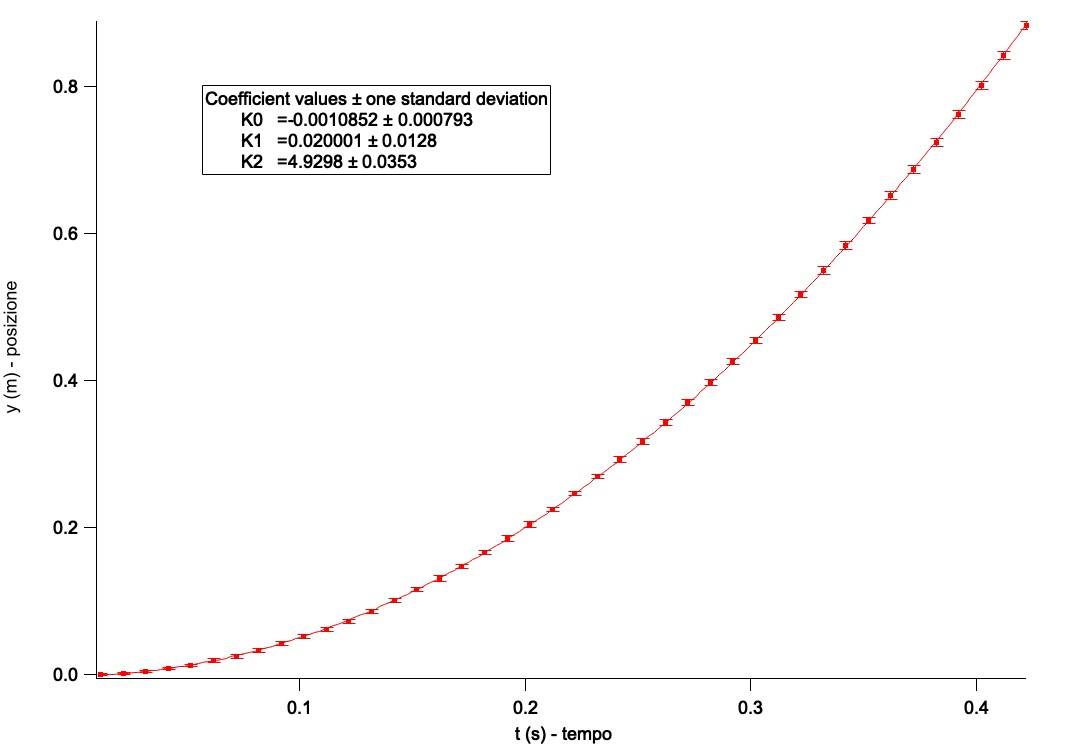
\includegraphics[width=170mm]{Immagini/Graph4 non comp.jpg}
\caption{\textit{{\footnotesize{Sulle ordinate compaiono i valori numerici di \textit{y(t)}, associati ai relativi errori  \textit{$\Delta y^{'}$}, mentre sulle ascisse ci sono gli istanti di tempo \textit{t}}}}}
\label{Grafico parabolico}
\end{figure}


I dati ottenuti tramite la regressione di potenza del secondo ordine (\textit{poli 3}), non sono compatibili con i valori teorici, fatta eccezione per $\displaystyle{\frac{g}{2}}$ :


\renewcommand{\theenumii}{\roman{enumii}}  
\begin{itemize}
    \itemsep0em 
    
        \item Posizione iniziale $y(0)$:
        
        \begin{tabular}{ccc}
        {$K_0 = -0.0010852 \pm 0.000793$} & & \small{(Non compatibile con il valore atteso $K_{0}$ $_{atteso}= 0.0000$)}\\
        \end{tabular}
        
    \end{itemize}
    \begin{itemize}
        \item Velocità iniziale $v(0)$:\\
        \begin{tabular}{ccccc}
        {$K_1 =  0.020001 \pm 0.0128$} & & & & \small{(Non compatibile con il valore atteso $K_{1}$ $_{atteso} = 0.0000$)}\\
        \end{tabular}
        
    \end{itemize}
      \begin{itemize}
          \item Coefficiente del termine quadratico, pari a $\displaystyle{\frac{g}{2}}$:\\ 
          \begin{tabular}{cccccc}
              {$K_2 =  4.9298 \pm 0.0353$} & & & & &\small{(Compatibile con il valore atteso $K_{2}$ $_{atteso}= 4.9033$)}\\
          \end{tabular}
         
      \end{itemize}
    \bigskip
Visto che \textit{posizione iniziale} e \textit{velocità iniziale} non sono compatibili con i valori attesi abbiamo corretto l'incompatibilità, isolando a destra il termine in relazione  quadratica con il tempo, mentre a sinistra, abbiamo ottenuto una nuova variabile $y_{new}$ in cui, la posizione $y$, è corretta dai termini $K_0$ e $ K_1\ t$, col rispettivo errore $\Delta y_{new}$: \\
L'equazione diventa quindi:
\begin{equation*}
\begin{aligned}
  & & y - K_0 - K_1\ t = K_0'+K_1'\ t+K_{2}'\ t^2
  &\quad{} 
  \end{aligned}
  \begin{aligned}
  & &\text{dove:\phantom{.......}} y_{new} = y - K_0 - K_1\ t 
  &
  \end{aligned}
\end{equation*}
L'errore su  $y_{new}$ è dato da
\begin{equation*}
 \Delta y_{new} = \Delta y + \Delta K_0 + \sqrt{\left(\frac{\Delta K_1}{K_1}\right)^2 + \left(\frac{\Delta t}{t}\right)^2}
 \end{equation*}


Facendo una nuova regressione di potenza del secondo ordine utilizzando i nuovi dati, otteniamo che le variabili $K_0'$, $K_1'$ e $K_2'$ sono tutte compatibili, come possiamo vedere in Figura \ref{Grafico parabolico}:
\bigskip
\bigskip

    \begin{figure}[h!]
\centering
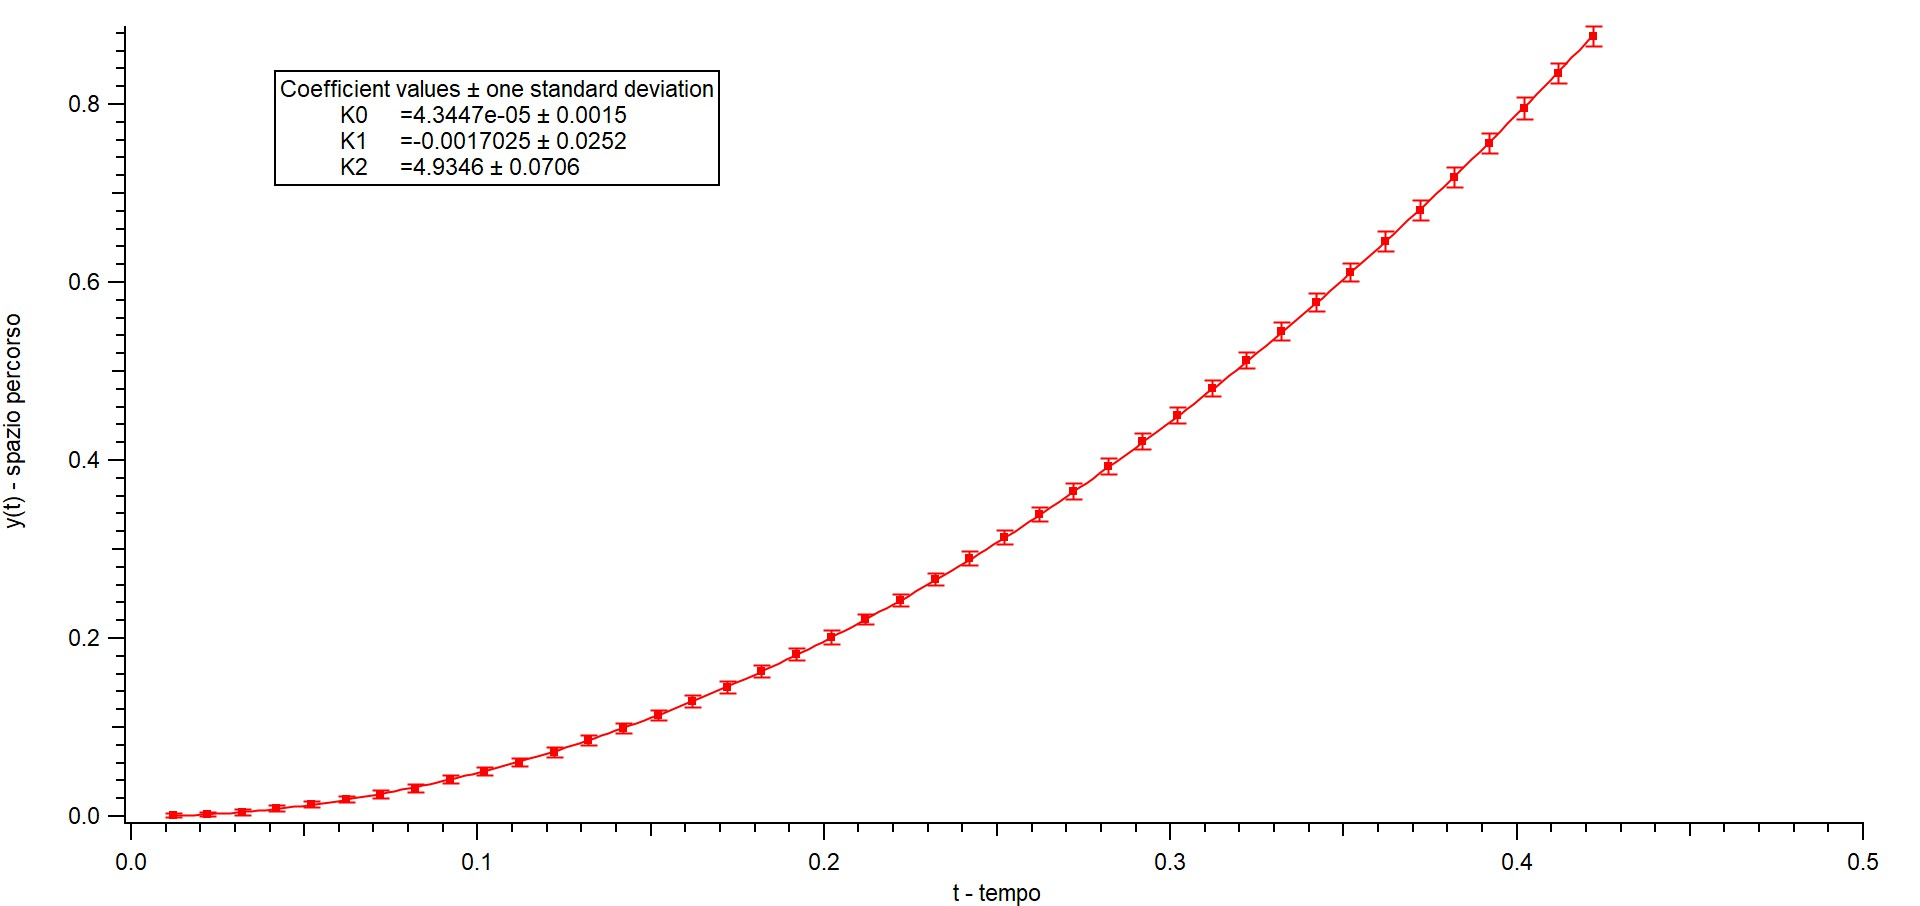
\includegraphics[width=170mm]{Immagini/Graph1.jpg}
\caption{\textit{{\footnotesize{Grafico $y_{new}(t)$: sul'asse asse $y$ sono riportati i valori di $y_{new}$ coi rispettivi errori, sull'asse $x$ il tempo}}}}
\label{Grafico parabolico}
\end{figure}




\newpage
\section{Regressione lineare}
Successivamente si è fatta una regressione lineare, partendo da $y_{new}= \frac{1}{2}\ g t^2$, approssimando posizione e velocità iniziali a $0$. Quello che ci si aspetta di trovare è che la posizione sia in relazione quadratica con il tempo:
\begin{equation*}
\begin{aligned}
  & y_{new}= \frac{1}{2}\ g\ t^2
  &\quad{} 
  \end{aligned}
  \begin{aligned}
  &&\text{passando ai logaritmi:\phantom{..}}& & \ln(y_{new})=\ln\left({\frac{1}{2}\ g}\right) +2\ln{t}
  &
  \end{aligned}
\end{equation*}
e come errore su $\ln({y_{new}})$: 
\begin{equation*}
    \Delta\ln{(y_{new})}=\frac{\Delta y_{new}}{y_{new}}\ 
\end{equation*}\\

\begin{table}[!h]
    \centering
    \begin{tabular}{|c|c|}
    \hline
    \multirow{2}{*}{\small Misura} 
    &\multirow{2}{*}{\small$\ln({y_{new}}) \pm\Delta\ln{(y_{new})}$\ $(m)$} 
     
    \\
    & 
    \\
    \hline
    \hline
       &   \\
    \hline
    \end{tabular}
        \caption{Caption}
        \label{tab:my_label}
\end{table}


 Tramite \textit{Igor Pro} si è ottenuto il seguente grafico:\\
   \begin{figure}[h!]
\centering
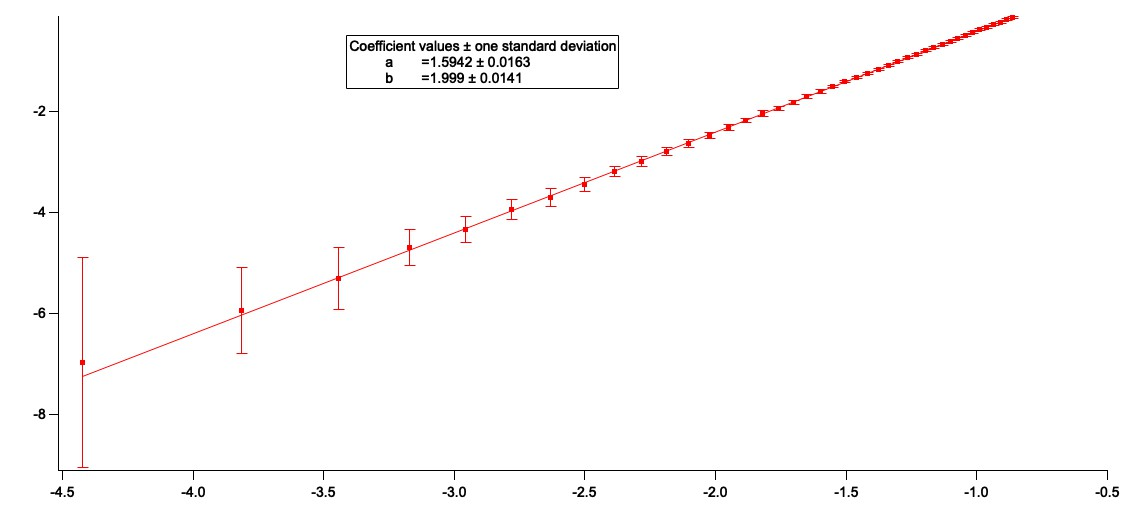
\includegraphics[width=170mm]{Immagini/GraphLn.jpg}
\caption{\textit{{\footnotesize{Grafico $\ln{(y_{new})}(\ln{t})$: sul'asse asse $y$ sono riportati i valori di $\ln{(y_{new})}$ coi rispettivi errori, sull'asse $x$ il $\ln{(t)}$}}}}
\label{Grafico logaritmico}
\end{figure}

Il valore di $b$ è compatibile col valore $2$, esponente del tempo nella formula usata in partenza.  Si è così dimostrato che vi è una relazione quadratica tra $y_{new}$ e $t$.





\newpage
\section{Calcolo dell'accelerazione di gravità}
A questo punto, dopo aver verificato che la posizione iniziale e finale sono approssimabili a $0$, e che la poszione è in relazione quadrtica con il tempo, possiamo creare un grafico lineare dei valori $y_{new}$, coi rispettivi errori, e del tempo al quadrato, così da essere in grado di ricavare il valore dell'accelerazione di gravità. 

\begin{figure}[h!]
\centering
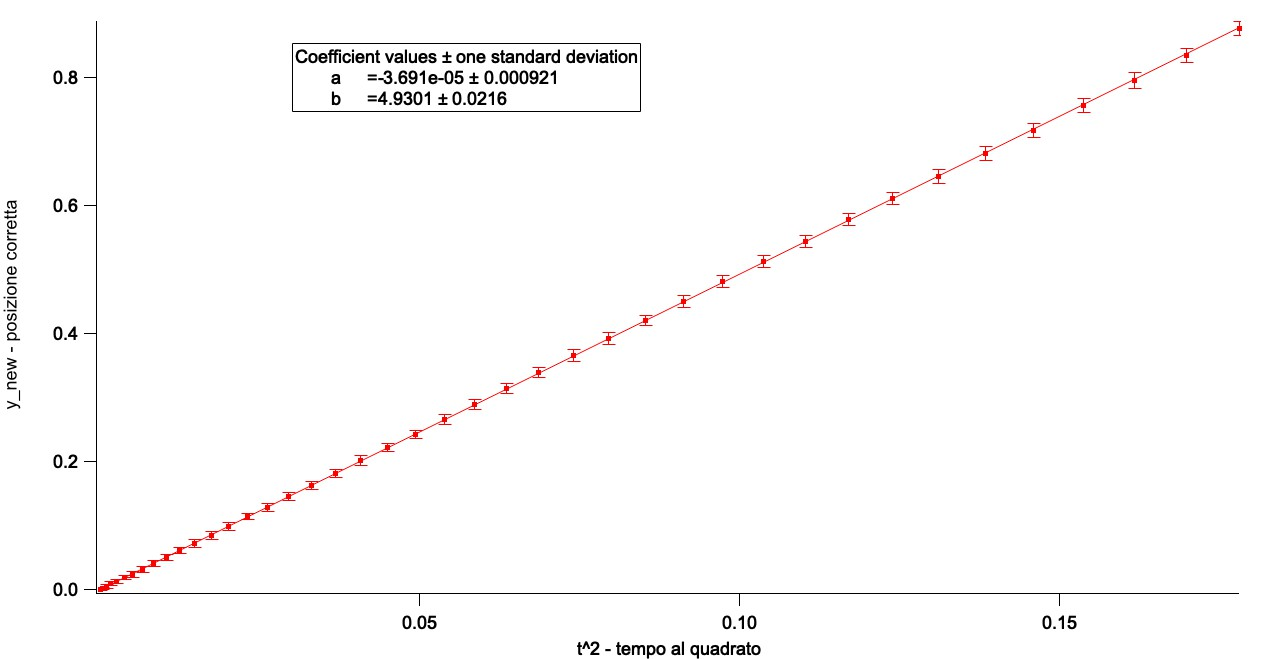
\includegraphics[width=170mm, height=80mm]{Immagini/Graph5 non comp.jpg}
\caption{\textit{{\footnotesize{Grafico $y_{new}(t^2)$: sull'asse asse $y$ sono riportati i valori di $y_{new}$ coi rispettivi errori, sull'asse $x$ il tempo al quadrato}}}}
\label{Grafico logaritmico}
\end{figure}



L'intercetta e la pendenza della retta ottenuta sono:
\begin{itemize}
    \item $a=-3.691\cdot 10^{-5}\pm 0.000921$
    \item$b=4.9301\pm 0.0216$
\end{itemize}
Dove $\displaystyle b=\frac{1}{2}\ g=(4.9301\pm 0.0216)$, da cui:
\begin{equation*}
    g=2 \ b=9.8602 \ \frac{m}{s^2}
\end{equation*}
e l'errore è
\begin{equation*}
    \Delta g=2\ \Delta b=0.04 \ \frac{m}{s^2}
\end{equation*}
Quindi l'accelerazione di gravità ottenuta sarebbe $g=(9.86\pm0.04)$ $\frac{m}{s^2}$.
Il valore $g$, ricavato a partire da $b$ , non risulta compatibile col valore standard poichè $|g-g_{tab}|> |\Delta g-\Delta g_{tab}|$. Questo è dovuto al fatto che ci potrebbero essere errori risultanti dalla configurazione e dalla qualità video dell'esperimento, che non erano sotto il nostro controllo. Per queste ragioni si è passati a due deviazioni standard con una confidenza del 95\%, e il grafico ottenuto è il seguente:
  \begin{figure}[h!]
\centering
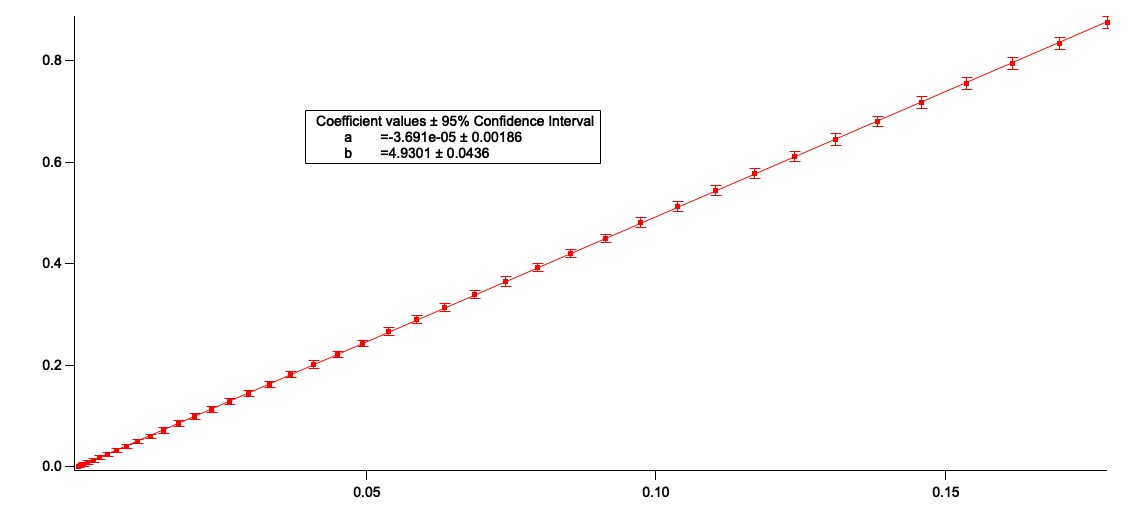
\includegraphics[width=170mm, height=80mm]{Immagini/Graphy_t^2.jpg}
\caption{\textit{{\footnotesize{Grafico $y_{new}(t^2)$: sull'asse asse $y$ sono riportati i valori di $y_{new}$ coi rispettivi errori, sull'asse $x$ il tempo al quadrato}}}}
\label{Grafico logaritmico}
\end{figure}

Si è infine passati al calcolo di $g$, utilizzando il valore di $b$ con un nuovo errore:
\begin{equation*}
    g=2 \ b=9.8602\ \frac{m}{s^2}
\end{equation*}
e l'errore è
\begin{equation*}
    \Delta g=2\ \Delta b=0.08\ \frac{m}{s^2}
\end{equation*}
Quindi il valore dell'accelerazione di gravità risultate è $g=(9.86\pm0.08)$ $\frac{m}{s^2}$
\section{Compatibilità}
Confrontiamo questo risultato col dato dell'accelerazione di gravità standard $g_{tab}=9,80665$, considerando quest'utimo senza errore:
\begin{equation*}
\begin{aligned}
  & |g-g_{tab}|=0.05335 \ \frac{m}{s^2}
  &\quad{} 
  \end{aligned}
  \begin{aligned}
  &&\text{,\phantom{..}}& & 
  |\Delta g-\Delta g_{tab}|=0.08\ \frac{m}{s^2}
  &
  \end{aligned}
\end{equation*}

Visto che $|g-g_{tab}|<< |\Delta g-\Delta g_{tab}|$, il valore trovato è compatibile col valore standard.





\section{Conclusioni}
La prima difficoltà è stata riscontrata nello stabilire tramite il programa di tracciamento le distanze metriche del video perchè, nonostante l'asta presentasse ogni 10cm un segno, questi erano tutt'altro che sottili, e ciò ha contribuito alle non compatibilità riscontrate successivamente. 

Anche in prossimità della fine della caduta è stato difficile prendere dei dati accurati, perchè non era chiaro quando la sfera colpisse il tavolo, quindi, per evitare di misurare ad urto avvenuto, abbiamo preso l'ultimo dato quando eravamo sicuri che fosse ancora in moto.

Infatti, nella prima regressione lineare, nè la velocità iniziale nè l'ordinata iniziale sono compatibili con i valori attesi di 0. Sono stati resi accettabili aumentando la tolleranza come mostrato nel paragrafo \ref{Agg. misure xconcl}\\

Per quanto riguarda la misura di $g$, inizialmente si era calcolato un errore relativo $\frac{\Delta g}{g}\approx 6\% $ ottenuto a partire da dei valori intermedi delle nostre misure. L'errore relativo che si ottinene dal valore finale dell'accelerazione di gravità ottenuto è:
\begin{equation*}
    \frac{\Delta g}{g}=\frac{0.08}{9.86}=0.8\%
\end{equation*}
risultato che differisce di un ordine di grandezza dal primo. Questo può essere dovuto al fatto che abbiamo cosiderato un errore specifico per ogni misura, in base alla definizione del frame, quindi alcune misure risultano più precise di altre. Inoltre sono state attuate le correzioni citate prima, per rendere compatibili  la posizione iniziale e la velocità iniziale. \\


Successivamente si è effettuata una regressione di potenza tra lo spazio e il tempo. L'esponente risulta pienamente compatibile con il valore atteso di 2, calcolando con una deviazione standard.
Per il calcolo di $g$, invece, si è usata una regressione lineare tra spazio percorso e tempo al quadrato, per la quale è stato necessario aumentare la cofidenza al 95\% (2 deviazioni standard) perchè il dato non era compatibile. \\

Nonostante tutti i risultati, alla fine, sono corretti, avremmo potuto migliorare le nostre stime agendo sulla calibrazione dello strumento di misura su Tracker, che  sicuramente è la fonte di errore maggiore. Probabimente considerando la distanza tra più di 2 segni sulla sbarra (ad esempio calibrando su $30cm$ invece di $10cm$), l'errore effettivo (non quello stimato) sarebbe calato e quindi avremmo avuto misure più attendibili.
Inoltre, date le imcompatibilità trovate, e anche l'errore molto piccolo risultante su $g$ può essere che gli errori sulle singole misure fossero stati sottostimati.





\newpage
\section{Tabella completa}
\begin{table}[!htb]
    \centering
    \centerline{\begin{tabular}{|c|c|c|c|c|c|c|c|}
    \hline
    \multirow{2}{*}{\small Misura} &\multirow{2}{*}{ $y$\ $(m)$}
    &\multirow{2}{*}{\small$\Delta pixel $}
    &\multirow{2}{*}{\small$\Delta y_{misurato}$\ $(m)$}
    &\multirow{2}{*}{\small$t$\ $(s)$} 
    &\multirow{2}{*}{\small$y_{new}\pm\Delta y_{new}$\ $(m)$}
    &\multirow{2}{*}{\small$\ln({y_{new}}) \pm\Delta\ln{(y_{new})}$\ $(m)$}
    &\multirow{2}{*}{\small$\ln{(t)}$\ $(s)$}\\ 
    
    &&&&&&&\\
\hline
\hline
    \footnotesize $1$ &\footnotesize $0.0001$ & $2$& &&&&\\
    \footnotesize $2$& \footnotesize$0.0020$  & $2$& &&&&\\
    \footnotesize $3 $& \footnotesize$0.0045$ & $3$& &&&&\\
    \footnotesize $4 $& \footnotesize$0.0090$ & $3$& &&&&\\
    \footnotesize $5 $& \footnotesize$0.0130$ & $3$& &&&&\\
    \footnotesize $6 $&\footnotesize$0.0195$  & $3$& &&&&\\
    \footnotesize $7 $&\footnotesize$0.0250$  & $4$& &&&&\\
    \footnotesize $8 $& \footnotesize$0.0325$ & $4$& &&&&\\
    \footnotesize $9 $&\footnotesize$0.0420$  & $3$& &&&&\\
    \footnotesize $10 $& \footnotesize$0.0515$& $3$& &&&&\\
    \footnotesize $11 $& \footnotesize$0.0620$& $2$& &&&&\\ 
    \footnotesize $12 $&\footnotesize $0.0730$& $4$& &&&&\\
    \footnotesize $13 $& \footnotesize$0.0865$& $4$& &&&&\\
    \footnotesize $14 $& \footnotesize$0.1005$& $3$& &&&&\\
    \footnotesize $15 $& \footnotesize$0.1160$& $2$& &&&&\\
    \footnotesize $16 $& \footnotesize$0.1315$& $4$& &&&&\\
    \footnotesize $17 $& \footnotesize$0.1475$& $3$& &&&&\\
    \footnotesize $18 $& \footnotesize$0.1660$& $3$& &&&&\\
    \footnotesize $19 $& \footnotesize$0.1850$& $3$& &&&&\\
    \footnotesize $20 $& \footnotesize$0.2045$& $4$& &&&&\\
    \footnotesize $21 $&\footnotesize $0.2250$& $1$& &&&&\\
    \footnotesize $22 $& \footnotesize$0.2465$& $2$& &&&&\\
    \footnotesize $23 $& \footnotesize$0.2700$& $2$& &&&&\\
    \footnotesize $24 $& \footnotesize$0.2935$& $4$& &&&&\\
    \footnotesize $25 $& \footnotesize$0.3180$& $3$& &&&&\\
    \footnotesize $26 $& \footnotesize$0.3435$& $2$& &&&&\\
    \footnotesize $27 $& \footnotesize$0.3700$& $4$& &&&&\\
    \footnotesize $28 $& \footnotesize$0.3975$& $3$& &&&&\\
    \footnotesize $29 $& \footnotesize$0.4260$& $2$& &&&&\\
    \footnotesize $30 $& \footnotesize$0.4550$& $2$& &&&&\\ 
    \footnotesize $31 $& \footnotesize$0.4865$& $3$& &&&&\\
    \footnotesize $32 $& \footnotesize$0.5180$& $2$& &&&&\\
    \footnotesize $33 $& \footnotesize$0.5500$& $3$& &&&&\\
    \footnotesize $34 $& \footnotesize$0.5835$& $3$& &&&&\\
    \footnotesize $35 $& \footnotesize$0.6175$& $2$& &&&&\\
    \footnotesize $36 $& \footnotesize$0.6520$& $4$& &&&&\\
    \footnotesize $37 $& \footnotesize$0.6875$& $3$& &&&&\\
    \footnotesize $38 $& \footnotesize$0.7245$& $3$& &&&&\\
    \footnotesize $39 $& \footnotesize$0.7625$& $3$& &&&&\\
    \footnotesize $40 $& \footnotesize$0.8020$& $4$& &&&&\\
    \footnotesize $41 $&\footnotesize $0.8420$& $2$& &&&&\\
    \footnotesize $42$&\footnotesize $0.8835$ & $2$& &&&&\\
\hline
\end{tabular}}
  \caption{Caption}
  \label{Tabella Completa}
\end{table}

\end{document}
